% Source: https://tex.stackexchange.com/a/638575/6880

\documentclass[12pt]{article}
\usepackage{tikz}
\usetikzlibrary{hobby}

\begin{document}
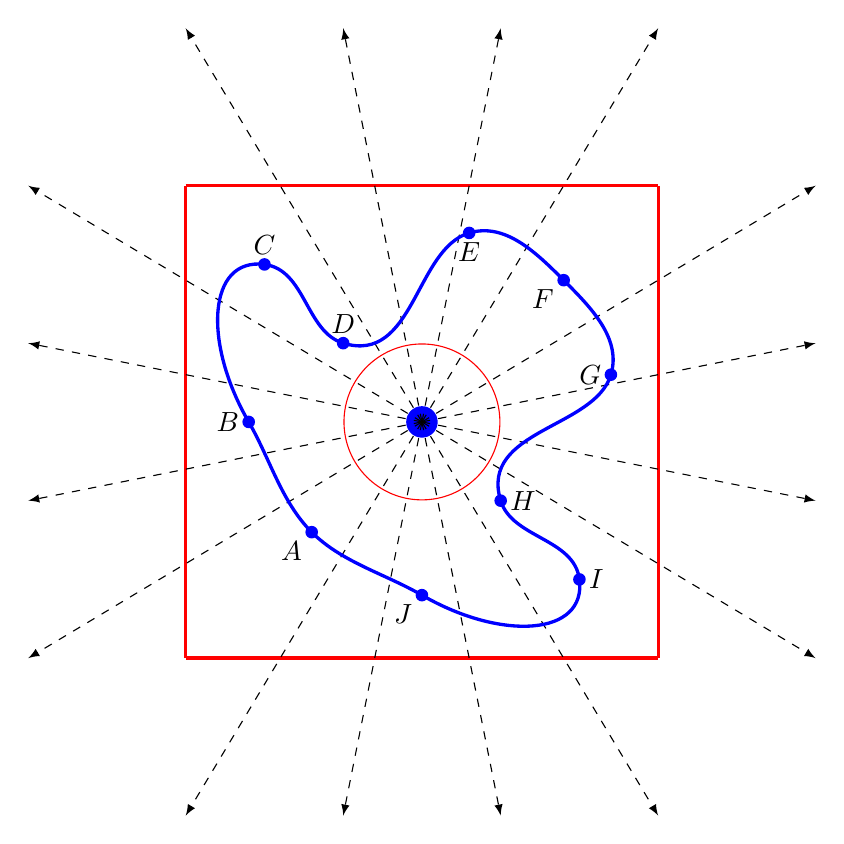
\begin{tikzpicture}[scale=2]
  \draw [red,very thick](4,2) --(7,2);
  \draw [red,very thick](4,5) --(7,5);
  \draw [red,very thick](7,2) --(7,5);
  \draw [red,very thick](4,2) --(4,5);

  \fill[blue,very thick] (5.5,3.5) circle(.1);
  %arrows on the right
  \draw [-latex][dashed] (5.5,3.5) --(8,5);
  \draw [-latex][dashed] (5.5,3.5) --(8,4);
  \draw [-latex][dashed] (5.5,3.5) --(8,3);
  \draw [-latex][dashed] (5.5,3.5) --(8,2);
   %arrows on the left
  \draw [-latex][dashed] (5.5,3.5) --(3,2);
  \draw [-latex][dashed] (5.5,3.5) --(3,3);
  \draw [-latex][dashed] (5.5,3.5) --(3,4);
  \draw [-latex][dashed] (5.5,3.5) --(3,5);
  %arrows at the bottom
  \draw [-latex][dashed] (5.5,3.5) --(4,1);
  \draw [-latex][dashed] (5.5,3.5) --(5,1);
  \draw [-latex][dashed] (5.5,3.5) --(6,1);
  \draw [-latex][dashed] (5.5,3.5) --(7,1);
  %arrows at the top
  \draw [-latex][dashed] (5.5,3.5) --(4,6);
  \draw [-latex][dashed] (5.5,3.5) --(5,6);
  \draw [-latex][dashed] (5.5,3.5) --(6,6);
  \draw [-latex][dashed] (5.5,3.5) --(7,6);
  %draw a circle
  \node(circle) [circle, inner sep=0.7cm, draw=red!120] at (5.5,3.5) {};

  \coordinate[label=below left:{$A$}] (A) at (4+0.8,2+0.8);
  \coordinate[label=left:{$B$}]       (B) at (4+0.4,2+1.5);
  \coordinate[label=above:{$C$}]      (C) at (4+0.5,2+2.5);
  \coordinate[label=above:{$D$}]      (D) at (4+1.0,2+2.0);
  \coordinate[label=below:{$E$}]      (E) at (4+1.8,2+2.7);
  \coordinate[label=below left:{$F$}] (F) at (4+2.4,2+2.4);
  \coordinate[label=left:{$G$}]       (G) at (4+2.7,2+1.8);
  \coordinate[label=right:{$H$}]      (H) at (4+2.0,2+1.0);
  \coordinate[label=right:{$I$}]      (I) at (4+2.5,2+0.5);
  \coordinate[label=below left:{$J$}] (J) at (4+1.5,2+0.4);

  \draw[blue,very thick] (A) to [closed, curve through = {(B) (C) (D) (E) (F) (G) (H) (I) (J)}] (A);

  \foreach \j in {A,...,J}{\fill[blue] (\j) circle (0.04);}

\end{tikzpicture}

\end{document}